\documentclass[12pt]{article}
\usepackage[left=1cm, right=1cm, top=2cm,bottom=1.5cm]{geometry} 

\usepackage[parfill]{parskip}
\usepackage[utf8]{inputenc}
\usepackage[T2A]{fontenc}
\usepackage[russian]{babel}
\usepackage{enumitem}
\usepackage[normalem]{ulem}
\usepackage{amsfonts, amsmath, amsthm, amssymb, mathtools}

\usepackage{fancyhdr}
\pagestyle{fancy}
\renewcommand{\headrulewidth}{1.5pt}
\renewcommand{\footrulewidth}{1pt}

\usepackage{graphicx}
\usepackage[figurename=Рис.]{caption} 
\usepackage{subcaption}
\usepackage{float}

%%Наименование папки откуда забирать изображения
\graphicspath{ {./images/} }

%%Изменение формата для ввода доказательства
\renewcommand{\proofname}{$\square$  \nopunct}
\renewcommand\qedsymbol{$\blacksquare$}

\addto\captionsrussian{%
	\renewcommand{\proofname}{$\square$ \nopunct}%
}
%% Римские цифры
\newcommand{\RN}[1]{%
	\textup{\uppercase\expandafter{\romannumeral#1}}%
}


\theoremstyle{definition}
\newtheorem{defn}{Опр:}
\newtheorem{rem}{Rm:}
\newtheorem{prop}{Утв.}
\newtheorem{exrc}{Упр.}
\newtheorem{lemma}{Лемма}
\newtheorem{theorem}{Теорема}
\newtheorem{corollary}{Следствие}

\newenvironment{cusdefn}[1]
{\renewcommand\thedefn{#1}\defn}
{\enddefn}



\DeclareRobustCommand{\divby}{%
	\mathrel{\text{\vbox{\baselineskip.65ex\lineskiplimit0pt\hbox{.}\hbox{.}\hbox{.}}}}%
}


\newcommand{\smallerrel}[1]{\mathrel{\mathpalette\smallerrelaux{#1}}}
\newcommand{\smallerrelaux}[2]{\raisebox{.1ex}{\scalebox{.75}{$#1#2$}}}

\newcommand{\smallin}{\smallerrel{\in}}
\newcommand{\smallnotin}{\smallerrel{\notin}}


\begin{document}
	\lhead{Математическая логика}
	\chead{Беклимишев Л.Д.}
	\rhead{Лекция - 2}
	
\section*{Аксиоматика теории множеств}

Равенство определяли следующим образом: $x = y \overset{\text{def}}{\Leftrightarrow} \forall z, (z \in x \Leftrightarrow z \in y)$.

Изучили следующие аксиомы:
\begin{enumerate}[label={(\arabic*)}]
	\item \textbf{Аксиома равенства:} $x =y$;
	\item \textbf{Аксиома пары:} $\{\,x,y\,\}$;
	\item \textbf{Аксиома объединения:} $\cup x$;
	\item \textbf{Аксиома степени:} $\mathcal{P}(x)$;
	\item \textbf{Аксиома выделения:} $\{\,z \in x \mid \varphi(z)\,\}$;
\end{enumerate}
	
Для аксиомы выделения можно добавить параметры $\Rightarrow$ получим $\{\,z \in x \mid \varphi(z,p_1,\dotsc,p_n)\,\}$, например $\{\,z \in \mathbb{R} \mid z < a\,\}$, где $a$ - параметр.
	
\begin{defn}
	$X \times Y = \{\,\langle u,v\rangle \mid u \in X \wedge v \in Y \,\}$ - \uwave{Декартово произведение}, $\langle u,v\rangle \in \mathcal{P}\big(\mathcal{P}(X \cup Y)\big)$.
\end{defn}
	
	
Почему $\langle u, v \rangle \in \mathcal{P}\big(\mathcal{P}(X \cup Y)\big)$ - ?
	
$\langle x,y \rangle = \big\{\{x,y\}, \{x\}\big\}$\\ 
$\{x\} \in \mathcal{P}(X) \Rightarrow \{x\} \in \mathcal{P}(X \cup Y) \Rightarrow \{x,y\} \in \mathcal{P}(X\cup Y)$ и $\{x\} \in \mathcal{P}(X\cup Y) \Rightarrow$\\ 
$\big\{\{x,y\}, \{x\} \big\} \in \mathcal{P}\big(\mathcal{P}(X\cup Y)\big)$
	
Формальная запись Декартова произведения $$X \times Y = \big\{\,z \in \mathcal{P}\big(\mathcal{P}(X\cup Y)\big) \mid \exists u, v \colon (z = \langle u, v \rangle \wedge u \in X \wedge y \in Y) \,\big\}$$

$z = \langle u, v \rangle \Leftrightarrow z = \big\{\{u,v\},\{v\} \big\} \Leftrightarrow \exists z_1, \exists z_2, (z_1 = \{u\} \wedge z_2 = \{u,v\} \wedge z = \{z_1, z_2\})$\\
$z_1 = \{u\} \Leftrightarrow \forall w, (w \in z_1 \Leftrightarrow w = u)$

\begin{defn}
	$R$ - \uwave{бинарное отношение} между $A$ и $B$, если $R \subseteq A \times B$.
\end{defn}	

\begin{figure}[H]
	\centering
	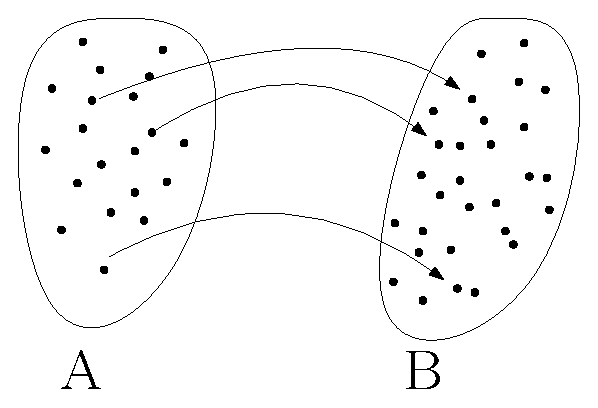
\includegraphics[width=0.25\textwidth]{ML2_1.eps}
	\caption{Бинарное отношение}
	\label{fig:2_1}
\end{figure}
	
\subsection*{Пример:}
$\langle x, y \rangle \in R \overset{\text{def}}{\Leftrightarrow} xRy$\\
$=_A \coloneqq \{\,\langle x,x,\rangle \mid x \in A\,\} \subseteq A \times A$ (равенство на $A$ или тождественная функция).
\newpage
\subsection*{Отношение эквивалентности:}

\begin{enumerate}[label={(\arabic*)}]
	\item \underline{Рефлексивное:} $\forall x \in A, (xRx)$;
	\item \underline{Транзитивное:} $\forall x, y, z \in A, (xRy \wedge yRz \Rightarrow xRz)$;
	\item \underline{Симметричное:} $\forall x, y \in A, (xRy \Rightarrow yRx)$;
\end{enumerate}

Можно разделять множества по классам эквивалентности: $x \in A \Rightarrow x_R \coloneqq \{\,y \in A \mid yRx\,\}$ (по А5), по определению $x \in x_R$.	

\begin{prop}
	$\forall x, y, (x_R = y_R \vee x_R \cap y_R = \varnothing)$.
\end{prop}

\begin{proof}
	$x \in A \Rightarrow x_R = \{y \in A \mid yRx\}$; пусть $x_1, x_2 \in A$, пусть $x_R^1 \cap x_R^2 \neq \varnothing \Rightarrow $ пусть $z \in x_R^1 \cap x_R^2 \Rightarrow x_1Rz \wedge x_2Rz \Rightarrow x_1Rx_2 \Rightarrow x_2Rx_1 \Rightarrow \forall z \colon x_2Rz \Rightarrow x_1Rz, \forall z \colon x_1Rz \Rightarrow x_2Rz \Rightarrow x_R^1 = x_R^2$, иначе $x_R^1 \cap x_R^2 = \varnothing$.
\end{proof}

$A/R$ - множество всех классов эквивалентности элементов множества $A$ по отношению $R$; $A/R$ - \uwave{фактор-множество}.

\begin{defn}
	\uwave{Фактор-множество} - $A/R = \{\,x_R \in \mathcal{P}(A) \mid x \in A\,\} = \{\,z \in \mathcal{P}(A) \mid \exists x\in A\colon x_R = z\,\}$, где $z = \{\,y \in A \mid yRx\,\}$ - по определению.
\end{defn}
	
$\bigsqcup A/R = A$ (все множество $A$ разбивается на классы эквивалентности).	

\subsection*{Целые числа $\mathbb{Z}$}
Пусть задали $\mathbb{N}$, как задать $\mathbb{Z}$ - ? \\
$\langle m,n \rangle$, где $m, n \in \mathbb{N}$; интуитивно: ``$m-n$'' $\Rightarrow \langle 1,2 \rangle	 \cong -1; \langle 2,3 \rangle	 \cong -1; \dotsc ;$

$=_\mathbb{Z}$ - \uwave{отношение эквивалентности} на $\mathbb{N}\times \mathbb{N}: \langle m_1, n_1 \rangle =_\mathbb{Z} \langle m_2, n_2 \rangle$ - ?\\
$$m_1 - n_1 = m_2 - n_2 \Leftrightarrow m_1 + n_2 = m_2 + n_1 \Rightarrow \langle m_1, n_1 \rangle =_\mathbb{Z} \langle m_2, n_2 \rangle \overset{\text{def}}{\Leftrightarrow} m_1 + n_2 = m_2 + n_1 \Rightarrow \mathbb{Z} \overset{\text{def}}{=} \big(\mathbb{N} \times \mathbb{N}/=_\mathbb{Z} \big)$$

\subsection*{Рациональные числа $\mathbb{Q}$}

Как задать $\mathbb{Q}$ - ?  $\dfrac{m}{n} \Rightarrow \langle m,n \rangle, m \in \mathbb{Z}, n \in \mathbb{N}\setminus\{0\} \Rightarrow \dfrac{m_1}{n_1} =_\mathbb{Q} \dfrac{m_2}{n_2} \Leftrightarrow m_1n_2 =_\mathbb{Z} n_1m_2 \Rightarrow$ \\
$\mathbb{Q} = \big(\mathbb{Z} \times (\mathbb{N}\setminus \{0\})/=_\mathbb{Q} \big)$
	
$=_\mathbb{Q}$ - \uwave{отношение эквивалентности} на $\mathbb{Z} \times (\mathbb{N}\setminus \{0\})$

\subsection*{Функции}

$f\colon A \rightarrow B$ - функция. $x \mapsto f(x)$ - соответствие, но в теории множеств все статично, все состоит из множеств, можем отождествить с графиком, то есть с парой $\Rightarrow f \subseteq A \times B \Rightarrow f = \{\,\langle x,f(x) \rangle \mid x \in A\,\}$, $f$ - частный случай бинарного отношения.

\subsection*{Свойства бинарных отношений:}
\begin{enumerate}[label={(\arabic*)}]
	\item \uwave{Функциональность:} $\forall x, y_1, y_2, (xRy_1 \wedge xRy_2 \Rightarrow y_1 = y_2)$;
	\item \uwave{Тотальность:} $\forall x \in A, \exists y \in B \colon xRy \Leftrightarrow \text{dom}R = A$;
	\item \uwave{Инъективность:} $\forall x_1, x_2, y, (x_1Ry \wedge x_2Ry \Rightarrow x_1 = x_2)$;
	\item \uwave{Сюръективность:} $\forall y \in B, \exists x \in A \colon xRy \Leftrightarrow \text{rng}R = B$;
\end{enumerate}

$\forall R, \exists R^{-1}\colon R^{-1} =\{\,\langle y,x \rangle \mid xRy \,\}, R^{-1} \subseteq B\times A$;

Можно заметить, что $R$ - функционально $\Leftrightarrow R^{-1}$ - инъективно, $R$ - тотально $\Leftrightarrow R^{-1}$ - сюръективно.

\begin{defn}
	$f \subseteq A\times B$ - \uwave{функция} из $A$ в $B$, если $f$ - тотальна и функциональна.	
\end{defn}

\begin{rem}
Если $f$ - только функциональна, то это \uwave{частичная функция}.
\end{rem}

\begin{defn}
	\uwave{Область определения} $\text{dom}R \overset{\text{def}}{=} \{\, x\in A \mid \exists y \in B \colon xRy\,\}$.
\end{defn}

\begin{defn}
	\uwave{Область значений} $\text{rng}R \overset{\text{def}}{=} \{\, y\in B \mid \exists x \in A \colon xRy\,\}$.
\end{defn}

\begin{defn}
	\uwave{Композицией} $R\cdot S$ двух отношений $R \colon A \rightarrow B$ и $S \colon B \rightarrow C$ называется $R\cdot S \subseteq A\times C$, такой что $xRSz \overset{\text{def}}{\Leftrightarrow} \exists y \in B \colon (xRy \wedge ySz)$.
\end{defn}

\begin{defn}
	$(f \circ g)(x) \overset{\text{def}}{=} f(g(x)), A \overset{g}{\rightarrow} B \overset{f}{\rightarrow} C \Rightarrow f\circ g \overset{\text{def}}{=} g \cdot f$.
\end{defn}

\end{document}